\documentclass[10pt,a4paper]{article}
\usepackage[utf8]{inputenc}
\usepackage[german]{babel}
\usepackage{mathrsfs}
\usepackage{amsmath}
\usepackage{physics}
\usepackage{amsfonts}
\usepackage{amssymb}
\usepackage{amsthm}
\usepackage{graphicx}
\usepackage[left=2cm,right=2cm,top=2cm,bottom=2cm]{geometry}

\begin{document}

\section{Aufgabe 2.1}

\subsection{Teil i}

Sei $z = a + ib \in \mathbb{C}$.
\begin{alignat*}{2}
&&  |z| & < 1 - \Re(z)\\
\Leftrightarrow \quad && \sqrt{\Re(z)^{2} + \Im(z)^{2}} & < 1 - \Re(z)\\
\Leftrightarrow \quad && \Re(z)^{2} + \Im(z)^{2} & < (1 - \Re(z))^{2} = 1 - 2\Re(z) + Re(z)^{2}\\
\Leftrightarrow \quad && \Im(z)^{2} & < 1 - 2\Re(z)\\
\Leftrightarrow \quad && \Re(z) & < \frac{1 - \Im(z)^{2}}{2} = -\frac{1}{2}\Im(z)^{2} + \frac{1}{2}\\
\end{alignat*}
\begin{figure}[h]
  \centering
  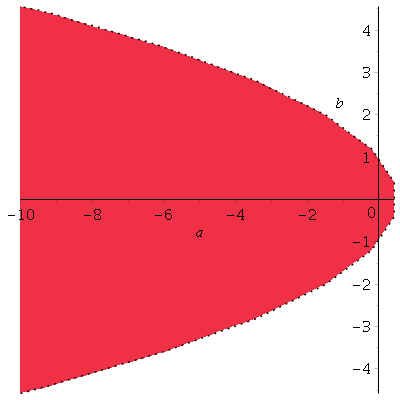
\includegraphics[width=200pt]{2_1_1}
  \caption{Nach links öffnende Parabel mit Stauchung $\frac{1}{2}$ und Scheitelpunkt $\frac{1}{2}$}
\end{figure}

\subsection{Teil ii}

Sei $z = a + ib \in \mathbb{C}$.
\begin{alignat*}{3}
&& \left| \frac{z - i}{z + i} \right|^{2} & = 4\\
\Leftrightarrow \quad && \left| a + i(b - 1) \right|^{2} & = 4 \cdot \left| a + i(b + 1) \right|^{2}\\
\Leftrightarrow \quad && a^{2} + (b - 1)^{2} & = 4 \cdot \left( a^{2} + (b + 1)^{2} \right)\\
\Leftrightarrow \quad && a^{2} + b^{2} - 2b + 1 & = 4a^{2} + 4b^{2} + 8b + 4\\
\Leftrightarrow \quad && 3a^{2} + 3b^{2} + 10b + 3 & = 0\\
\Leftrightarrow \quad && a^{2} + b^{2} + \frac{10}{3}b + 1 & = 0\\
\Leftrightarrow \quad && a^{2} + b^{2} + 2\frac{5}{3}b + \left( \frac{5}{3} \right)^{2} - \left( \frac{5}{3} \right)^{2} + 1 & = 0 \quad \textit{Quadratische Ergänzung}\\
\Leftrightarrow \quad && a^{2} + \left( b + \frac{5}{3} \right)^{2} - \frac{16}{9} & = 0\\
\Leftrightarrow \quad && a^{2} + \left( b + \frac{5}{3} \right)^{2} & = \left( \frac{4}{3} \right)^{2}\\
\end{alignat*}
\begin{figure}[h]
  \centering
  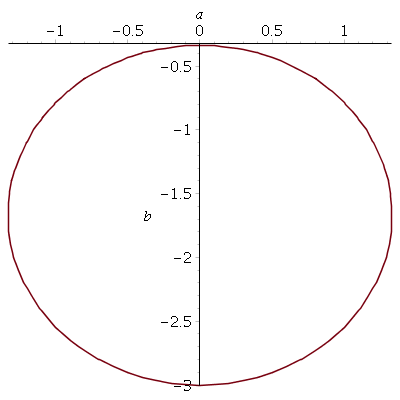
\includegraphics[width=200pt]{2_1_2}
  \caption{Ein Kreis mit Mittelpunkt $-\frac{5}{3}i$ und Radius $\frac{4}{3}$}
\end{figure}

\section{Aufgabe 2.2}

\subsection{Teil i}

Sei $n \in \mathbb{N}$ und $r \in \{ 0, 1, 2, 3 \}$.
\begin{equation}
  i^{4n + r} = i^{4n} \cdot i^{r} = i^{2^{2^{n}}} \cdot i^{r} = (-1)^{2^{n}} \cdot i^{r} = i^{r}
\end{equation}

\begin{align*}
  \sum_{n = 1}^{\infty} \frac{i^{n}}{n} & = \sum_{n = 0}^{\infty} \left( \frac{i^{4n + 1}}{4n + 1} + \frac{i^{4n + 2}}{4n + 2} + \frac{i^{4n + 3}}{4n + 3} + \frac{i^{4n + 4}}{4n + 4} \right)\\
                                        & = \sum_{n = 0}^{\infty} \left( \frac{i^{1}}{4n + 1} + \frac{i^{2}}{4n + 2} + \frac{i^{3}}{4n + 3} + \frac{i^{4}}{4n + 4} \right)\\
                                        & = \sum_{n = 0}^{\infty} \left( \frac{i}{4n + 1} + \frac{-1}{4n + 2} + \frac{-i}{4n + 3} + \frac{1}{4n + 4} \right)\\
                                        & = \sum_{n = 0}^{\infty} \frac{i(4n + 2)(4n + 3)(4n + 4) - (4n + 1)(4n + 3)(4n + 4) - i(4n + 1)(4n + 2)(4n + 4) + (4n + 1)(4n + 2)(4n + 3)}{(4n + 1)(4n + 2)(4n + 3)(4n + 4)}\\
                                        & = \sum_{n = 0}^{\infty} \frac{2i(4n + 2)(4n + 4) - 2(4n + 1)(4n + 3)}{(4n + 1)(4n + 2)(4n + 3)(4n + 4)}\\
                                        & = -2 \sum_{n = 0}^{\infty} \left( \frac{1}{(4n + 2)(4n + 4)} \right) + 2i \sum_{n = 0}^{\infty} \left( \frac{1}{(4n + 1)(4n + 3)} \right)\\
                                        & = -2 \sum_{n = 0}^{\infty} \left( \frac{1}{16n^{2} + 24n + 8} \right) + 2i \sum_{n = 0}^{\infty} \left( \frac{1}{16n^{2} + 16n + 3} \right)\\
\end{align*}
Die Summanden beider Summen sind jeweils kleiner als die Summanden der Reihe
$\sum_{n = 1}^{\infty} \frac{1}{n^{2}}$, die konvergiert, sodass diese beiden
Reihen ebenfalls konvergieren nach Majorantenkriterium und die ursprüngliche
Reihe ebenso. Maple sagt, dass der Grenzwert $-\frac{1}{2}\log(2) + \frac{1}{4}\pi i$ ist.

\subsection{Teil ii}

Sei $a_{k}$ das $k$-te Element der zu untersuchenden Reihe.
\begin{equation*}
  \left| \frac{a_{k + 1}}{a_{k}} \right| = \left| \frac{\frac{2 + i}{(1 + i)^{2(n + 1)}}}{\frac{2 + i}{(1 + i)^{2n}}} \right| = \left| \frac{(1 + i)^{2n}}{(1 + i)^{2(n + 1)}} \right| = \left| \frac{1}{(1 + i)^{2}} \right| = \left| \frac{1}{2i} \right| = \left| -\frac{1}{2}i \right| = \frac{1}{2}
\end{equation*}
\begin{equation*}
  \limsup_{k \to \infty} \left| \frac{a_{k + 1}}{a_{k}} \right| = \limsup_{k \to \infty} \frac{1}{2} < 1
\end{equation*}
Die Reihe konvergiert also nach Quotientenkriterium. Maple sagt, dass der
Grenzwert $-i$ ist.

\section{Aufgabe 2.3}

\subsection{Teil a}

Beweis per Induktion.

\begin{proof}
  Sei $n = 1$. Dann ist
  \begin{equation*}
    \left( \prod_{j = 1}^{n} f_{j} \right)^{'}(z_{0}) = f_{1}^{'}(z_{0}) = \sum_{j = 1}^{n} f_{j}^{'}(z_{0}) \prod_{i \ne j}^{n} f_{i}(z_{0})
  \end{equation*}

  Sei $n \ge 1$, sodass
  $\left( \prod_{j = 1}^{n - 1} f_{j} \right)^{'}(z_{0}) = \sum_{j = 1}^{n - 1}
  f_{j}^{'}(z_{0}) \prod_{i \ne j}^{n - 1} f_{i}(z_{0})$. Dann gilt
  \begin{align*}
    \left( \prod_{j = 1}^{n} f_{j} \right)^{'}(z_{0}) & = \left( f_{n} \cdot \prod_{j = 1}^{n - 1} f_{j} \right)^{'}(z_{0})\\
                                                      & = \left( f_{n}^{'} \cdot \prod_{j = 1}^{n - 1} f_{j} \right)(z_{0}) + \left( f_{n} \cdot \left( \prod_{j = 1}^{n - 1} f_{j} \right)^{'} \right)(z_{0})\\
                                                      & = \left( f_{n}^{'} \cdot \prod_{j = 1}^{n - 1} f_{j} \right)(z_{0}) + \left( f_{n} \cdot \left( \sum_{j = 1}^{n - 1} f_{j}^{'} \prod_{i \ne j}^{n - 1} f_{i} \right) \right)(z_{0})\\
                                                      & = \left( f_{n}^{'} \cdot \prod_{i \ne n}^{n} f_{i} \right)(z_{0}) +  \left( \sum_{j = 1}^{n - 1} f_{j}^{'} \prod_{i \ne j}^{n} f_{i} \right) (z_{0})\\
                                                      & = \sum_{j = 1}^{n} f_{j}^{'}(z_{0}) \prod_{i \ne j}^{n} f_{i}^{'}(z_{0})
  \end{align*}
\end{proof}

\subsection{Teil b}

\begin{proof}
  Wir betrachten zuerst $\frac{1}{g}$.
  \begin{align*}
    \left( \frac{1}{g} \right)^{'}(z_{0}) & = \lim_{z \to z_{0}} \frac{\frac{1}{g(z)} - \frac{1}{g(z_{0})}}{z - z_{0}}\\
                                          & = \lim_{z \to z_{0}} \frac{\frac{g(z_{0}) - g(z)}{g(z)g(z_{0})}}{z - z_{0}}\\
                                          & = - \lim_{z \to z_{0}} \frac{1}{g(z)g(z_{0})} \cdot \frac{g(z) - g(z_{0})}{z - z_{0}}\\
                                          & = - \lim_{z \to z_{0}} \frac{1}{g(z)g(z_{0})} \cdot \lim_{z \to z_{0}} \frac{g(z) - g(z_{0})}{z - z_{0}}\\
                                          & = -\frac{1}{(g(z_{0}))^{2}} \cdot g^{'}(z_{0})\\
                                          & = -\frac{g^{'}(z_{0})}{(g(z_{0})^{2})}
  \end{align*}

  \begin{align*}
    \left( \frac{f}{g} \right)^{'}(z_{0}) & = \left( f \cdot \frac{1}{g} \right)^{'}(z_{0})\\
                                          & = f^{'}(z_{0})\left( \frac{1}{g} \right)(z_{0}) + f(z_{0})\left( \frac{1}{g} \right)^{'}(z_{0})\\
                                          & = \left( \frac{f^{'}(z_{0})g(z_{0})}{(g(z_{0}))^{2}} \right) + f(z_{0})\left( -\frac{g^{'}(z_{0})}{(g(z_{0})^{2})} \right)\\
                                          & = \frac{f^{'}(z_{0})g(z_{0}) - f(z_{0})g^{'}(z_{0})}{(g(z_{0}))^{2}}
  \end{align*}
\end{proof}

\section{Aufgabe 2.4}

\begin{proof}
  $(i) \Rightarrow (ii)$: Sei $(X, \delta)$ zusammenhängend und $M \subset X$
  offen und abgeschlossen in $X$. Da $M$ abgeschlossen ist, ist
  $M^{\complement}$ offen. Wir haben also eine Zerlegung von $X$ in zwei offene
  Mengen gefunden, sodass $M \cap M^{\complement} = \emptyset$. Nach der
  Definition von zusammenhängend ist $M = X$ oder $M = \emptyset$.

  $(ii) \Rightarrow (iii)$: Sei $f : X \to \{ 0, 1 \}$ eine stetige
  Funktion. Definiere $M := \{ x \in X \mid f(x) = 0 \}$. Wenn $M$ leer ist, ist
  $f \equiv 1$. Sei also $M \ne \emptyset$ und $x \in M$. Da $f$ stetig ist,
  gibt es eine offene Kugel $B_{r}(x)$ auf der
  $|f(y) - f(x)| < \frac{1}{2}\ \forall y \in B_{r}(x)$. Es folgt
  $f|_{B_{r}(x)} \equiv 0 \Rightarrow B_{r}(x) \subset M$. $M$ ist somit
  offen. Da $f$ eine Funktion, also total, ist, ist
  $M^{\complement} = \{ x \in X \mid f(x) = 1 \}$. Nach derselben Argumentation
  wie für $M$ ist auch $M^{\complement}$ offen und daher $M$ abgeschlossen. Nach
  Vorraussetzung und der Annahme, dass $M$ nicht leer ist, muss $M = X$
  sein. $f$ ist also die $0$-Funktion und wiederum konstant.

  $(iii) \Rightarrow (i)$: Seien $U, V \subset X$ offen in $X$ mit
  $U \cap V = \emptyset$ und $U \cup V = X$. Wenn $U = \emptyset$, ist schon
  $V = X$. Sei also $U \ne \emptyset$. Wir betrachten die Indikatorfunktion
  $f = \mathcal{I}(U)$ von $U$. Da $U$ und $V$ eine offene Zerlegung und $f$ auf
  beiden Mengen konstant ist, ist $f$ stetig (Es gibt um jeden Punkt eine Kugel
  auf der $f$ denselben Wert annimmt). Damit ist $f$ nach Vorraussetzung
  konstant auf $X$. Da wir weiterhin angenommen haben, dass $U \ne \emptyset$,
  muss $f \equiv 1$ sein und $V = \emptyset$. $X$ ist also zusammenhängend.
\end{proof}

\end{document}